\documentclass{article}\usepackage[]{graphicx}\usepackage[]{color}
%% maxwidth is the original width if it is less than linewidth
%% otherwise use linewidth (to make sure the graphics do not exceed the margin)
\makeatletter
\def\maxwidth{ %
  \ifdim\Gin@nat@width>\linewidth
    \linewidth
  \else
    \Gin@nat@width
  \fi
}
\makeatother

\definecolor{fgcolor}{rgb}{0.345, 0.345, 0.345}
\newcommand{\hlnum}[1]{\textcolor[rgb]{0.686,0.059,0.569}{#1}}%
\newcommand{\hlstr}[1]{\textcolor[rgb]{0.192,0.494,0.8}{#1}}%
\newcommand{\hlcom}[1]{\textcolor[rgb]{0.678,0.584,0.686}{\textit{#1}}}%
\newcommand{\hlopt}[1]{\textcolor[rgb]{0,0,0}{#1}}%
\newcommand{\hlstd}[1]{\textcolor[rgb]{0.345,0.345,0.345}{#1}}%
\newcommand{\hlkwa}[1]{\textcolor[rgb]{0.161,0.373,0.58}{\textbf{#1}}}%
\newcommand{\hlkwb}[1]{\textcolor[rgb]{0.69,0.353,0.396}{#1}}%
\newcommand{\hlkwc}[1]{\textcolor[rgb]{0.333,0.667,0.333}{#1}}%
\newcommand{\hlkwd}[1]{\textcolor[rgb]{0.737,0.353,0.396}{\textbf{#1}}}%
\let\hlipl\hlkwb

\usepackage{framed}
\makeatletter
\newenvironment{kframe}{%
 \def\at@end@of@kframe{}%
 \ifinner\ifhmode%
  \def\at@end@of@kframe{\end{minipage}}%
  \begin{minipage}{\columnwidth}%
 \fi\fi%
 \def\FrameCommand##1{\hskip\@totalleftmargin \hskip-\fboxsep
 \colorbox{shadecolor}{##1}\hskip-\fboxsep
     % There is no \\@totalrightmargin, so:
     \hskip-\linewidth \hskip-\@totalleftmargin \hskip\columnwidth}%
 \MakeFramed {\advance\hsize-\width
   \@totalleftmargin\z@ \linewidth\hsize
   \@setminipage}}%
 {\par\unskip\endMakeFramed%
 \at@end@of@kframe}
\makeatother

\definecolor{shadecolor}{rgb}{.97, .97, .97}
\definecolor{messagecolor}{rgb}{0, 0, 0}
\definecolor{warningcolor}{rgb}{1, 0, 1}
\definecolor{errorcolor}{rgb}{1, 0, 0}
\newenvironment{knitrout}{}{} % an empty environment to be redefined in TeX

\usepackage{alltt}
\usepackage{amsmath}
\usepackage{makecell}
\setcellgapes{5pt}
\usepackage{graphics}
\usepackage{multicol}
\usepackage[cm]{fullpage}
\graphicspath{ {./images/} }
\usepackage{titling}
\usepackage[table]{xcolor}
\usepackage[mathscr]{euscript}
\usepackage{mathrsfs}
\usepackage{ulem, cancel}
\usepackage{boldline}

\title{COSC 6323 - Statistical Methods in Research\\Project Phase - 2\\}

\author{%
    Members: Team-8 \\\\
    1. Farah Naz Chowdhury,    \texttt{ID:1798957}, \texttt{fchowdhury4@uh.edu}      \vspace{2pt} \\
    2. Md Rafiqul Islam Rabin, \texttt{ID:1797648}, \texttt{mrabin@central.uh.edu}   \vspace{2pt} \\
    3. S M Salah Uddin Kadir , \texttt{ID:1800503}, \texttt{ssalahuddinkadir@uh.edu} \vspace{2pt} \\
}

\date{April 05, 2019.}
\IfFileExists{upquote.sty}{\usepackage{upquote}}{}
\begin{document}

\maketitle
\par{\textbf{Contributions}: Contribution paragraph goes here.}

%Fig. 4
\newpage
\section*{\underline{Fig. 4:}}
\begin{center}
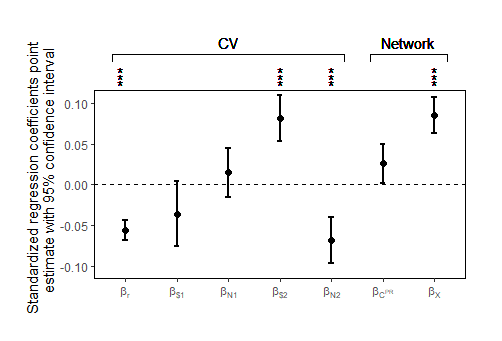
\includegraphics[scale=1.0]{4.png}
\newline
\par{\textbf{Fig. 4. Career cross-sectional regression model.}}
\end{center}
\subsection*{\underline{Description of figure content:}}
\par{
Descriptions goes here.
}
\subsection*{\underline{Observations, conclusions, and hypotheses:}}
\par{
observations goes here.
}

%Table S2
\newpage
\section*{\underline{Table S2:}}
\begin{table}[h!]
  \begin{center}
  \label{tab:table1}
  \begin{tabular}{l c c c c c}
  
    \hline
    \hline
    
    {} & {(a)} & {(b)} & {(c)} & {(d)} & {(e)}  \\
    {} & {$\mathscr{C}^{PR}$} & {$\mathscr{C}^{B}$} & {$\mathscr{C}^{D}$} & {$\cancel{\beta_{N1},\beta_{N2}}$} & {$\cancel{\beta_{r}}$}  \\
    
    \hline
    
    \textbf {CV parameters}\\
    
    \rowcolor{gray!33}
    Departmental rank, $\beta_{r}$ 
    & -0.000*** & -0.000***  & -0.000*** & -0.000*** & -0.000*** \\
    {} 
    & (0.000)   & (0.000)    & (0.000)   & (0.000)   & (0.000) \\
    
    \rowcolor{gray!33}
    Productivity (\textit{h}-index), $\beta_{h}$ 
    & -0.000*** & -0.000***  & -0.000*** & -0.000*** & -0.000*** \\
    {} 
    & (0.000)   & (0.000)    & (0.000)   & (0.000)   & (0.000) \\
    
    \rowcolor{gray!33}
    Total NSF funding, $\beta_{\$1}$ 
    & -0.000*** & -0.000***  & -0.000*** & -0.000*** & -0.000*** \\
    {} 
    & (0.000)   & (0.000)    & (0.000)   & (0.000)   & (0.000) \\
    
    \rowcolor{gray!33}
    {\#} of NSF grants, $\beta_{N1}$ 
    & -0.000*** & -0.000***  & -0.000*** & -0.000*** & -0.000*** \\
    {} 
    & (0.000)   & (0.000)    & (0.000)   & (0.000)   & (0.000) \\
    
    \rowcolor{gray!33}
    Total NIH funding, $\beta_{\$2}$ 
    & -0.000*** & -0.000***  & -0.000*** & -0.000*** & -0.000*** \\
    {} 
    & (0.000)   & (0.000)    & (0.000)   & (0.000)   & (0.000) \\
    
    \rowcolor{gray!33}
    {\#} of NIH grants, $\beta_{N2}$ 
    & -0.000*** & -0.000***  & -0.000*** & -0.000*** & -0.000*** \\
    {} 
    & (0.000)   & (0.000)    & (0.000)   & (0.000)   & (0.000) \\
    
    \hline
    
    \textbf {Network parameters}\\
    
    \rowcolor{gray!33}
    PageRank centrality, $\beta_{\mathscr{C}^{PR}}$ 
    & -0.000*** & -0.000***  & -0.000*** & -0.000*** & -0.000*** \\
    {} 
    & (0.000)   & (0.000)    & (0.000)   & (0.000)   & (0.000) \\
    
    \rowcolor{gray!33}
    Betweenness centrality, $\beta_{\mathscr{C}^{B}}$ 
    & -0.000*** & -0.000***  & -0.000*** & -0.000*** & -0.000*** \\
    {} 
    & (0.000)   & (0.000)    & (0.000)   & (0.000)   & (0.000) \\
    
    \rowcolor{gray!33}
    Degree centrality, $\beta_{\mathscr{C}^{D}}$ 
    & -0.000*** & -0.000***  & -0.000*** & -0.000*** & -0.000*** \\
    {} 
    & (0.000)   & (0.000)    & (0.000)   & (0.000)   & (0.000) \\
    
    \rowcolor{gray!33}
    Cross-disciplinarity, $\beta_{\chi}$ 
    & -0.000*** & -0.000***  & -0.000*** & -0.000*** & -0.000*** \\
    {} 
    & (0.000)   & (0.000)    & (0.000)   & (0.000)   & (0.000) \\
    
    \hline
    
    \rowcolor{gray!33} 
    Discipline ($\mathscr{O}$) dummy & $\textit{Y}$ & $\textit{Y}$ & $\textit{Y}$ & $\textit{Y}$ & $\textit{Y}$ \\
    
    \rowcolor{gray!33} 
    5-year cohort $(y{^0_i{_,}}_{5})$ dummy & $\textit{Y}$ & $\textit{Y}$ & $\textit{Y}$ & $\textit{Y}$ & $\textit{Y}$ \\
    
    \rowcolor{gray!33} 
    Constant 
    & -0.000*** & -0.000***  & -0.000*** & -0.000*** & -0.000*** \\
    {} 
    & (0.000)   & (0.000)    & (0.000)   & (0.000)   & (0.000) \\
    
    \hline
    
    \rowcolor{gray!33} 
    $\textit{n}$
    & 3900 & 3387 & 3900 & 3900 & 3900 \\
    
    \rowcolor{gray!33} 
    adj. ${R^2}$ 
    & 0.882 & 0.873 & 0.883 & 0.882 & 0.881 \\
    
    \hline
    \hline
    
    Standard errors in parentheses, listed below coefficient estimate. \\
    {* $\textit{p}$ $\leq$ .05, ** $\textit{p}$ $\leq$ .01, *** $\textit{p}$ $\leq$ .001}
    
  \end{tabular}
  \end{center}
\end{table}
\begin{center}
\par{\textbf{Table S2. Career data set: Pooled cross-sectional model.}}
\end{center}
\subsection*{\underline{Description of figure content:}}
\par{
Descriptions goes here.
}
\subsection*{\underline{Observations, conclusions, and hypotheses:}}
\par{
observations goes here.
}

%Table S3
\newpage
\section*{\underline{Table S3:}}
\begin{table}[h!]
  \begin{center}
  \label{tab:table1}
  \begin{tabular}{l c c c c c}
  
    \hline
    \hline
    
    {} & {(a)} & {(b)} & {(c)} & {(d)} & {(e)}  \\
    {} & {$\mathscr{C}^{PR}$} & {$\mathscr{C}^{B}$} & {$\mathscr{C}^{D}$} & {$\cancel{\beta_{N1},\beta_{N2}}$} & {$\cancel{\beta_{r}}$}  \\
    
    \hline
    
    \textbf {CV parameters}\\
    
    \rowcolor{gray!33}
    Departmental rank, $\beta_{r}$ 
    & -0.000*** & -0.000***  & -0.000*** & -0.000*** & -0.000*** \\
    {} 
    & (0.000)   & (0.000)    & (0.000)   & (0.000)   & (0.000) \\
    
    \rowcolor{gray!33}
    Productivity (\textit{h}-index), $\beta_{h}$ 
    & -0.000*** & -0.000***  & -0.000*** & -0.000*** & -0.000*** \\
    {} 
    & (0.000)   & (0.000)    & (0.000)   & (0.000)   & (0.000) \\
    
    \rowcolor{gray!33}
    Total NSF funding, $\beta_{\$1}$ 
    & -0.000*** & -0.000***  & -0.000*** & -0.000*** & -0.000*** \\
    {} 
    & (0.000)   & (0.000)    & (0.000)   & (0.000)   & (0.000) \\
    
    \rowcolor{gray!33}
    {\#} of NSF grants, $\beta_{N1}$ 
    & -0.000*** & -0.000***  & -0.000*** & -0.000*** & -0.000*** \\
    {} 
    & (0.000)   & (0.000)    & (0.000)   & (0.000)   & (0.000) \\
    
    \rowcolor{gray!33}
    Total NIH funding, $\beta_{\$2}$ 
    & -0.000*** & -0.000***  & -0.000*** & -0.000*** & -0.000*** \\
    {} 
    & (0.000)   & (0.000)    & (0.000)   & (0.000)   & (0.000) \\
    
    \rowcolor{gray!33}
    {\#} of NIH grants, $\beta_{N2}$ 
    & -0.000*** & -0.000***  & -0.000*** & -0.000*** & -0.000*** \\
    {} 
    & (0.000)   & (0.000)    & (0.000)   & (0.000)   & (0.000) \\
    
    \hline
    
    \textbf {Network parameters}\\
    
    \rowcolor{gray!33}
    PageRank centrality, $\beta_{\mathscr{C}^{PR}}$ 
    & -0.000*** & -0.000***  & -0.000*** & -0.000*** & -0.000*** \\
    {} 
    & (0.000)   & (0.000)    & (0.000)   & (0.000)   & (0.000) \\
    
    \rowcolor{gray!33}
    Betweenness centrality, $\beta_{\mathscr{C}^{B}}$ 
    & -0.000*** & -0.000***  & -0.000*** & -0.000*** & -0.000*** \\
    {} 
    & (0.000)   & (0.000)    & (0.000)   & (0.000)   & (0.000) \\
    
    \rowcolor{gray!33}
    Degree centrality, $\beta_{\mathscr{C}^{D}}$ 
    & -0.000*** & -0.000***  & -0.000*** & -0.000*** & -0.000*** \\
    {} 
    & (0.000)   & (0.000)    & (0.000)   & (0.000)   & (0.000) \\
    
    \rowcolor{gray!33}
    Cross-disciplinarity, $\beta_{\chi}$ 
    & -0.000*** & -0.000***  & -0.000*** & -0.000*** & -0.000*** \\
    {} 
    & (0.000)   & (0.000)    & (0.000)   & (0.000)   & (0.000) \\
    
    \hline
    
    \rowcolor{gray!33} 
    Discipline ($\mathscr{O}$) dummy & $\textit{Y}$ & $\textit{Y}$ & $\textit{Y}$ & $\textit{Y}$ & $\textit{Y}$ \\
    
    \rowcolor{gray!33} 
    5-year cohort $(y{^0_i{_,}}_{5})$ dummy & $\textit{Y}$ & $\textit{Y}$ & $\textit{Y}$ & $\textit{Y}$ & $\textit{Y}$ \\
    
    \rowcolor{gray!33} 
    Constant 
    & -0.000*** & -0.000***  & -0.000*** & -0.000*** & -0.000*** \\
    {} 
    & (0.000)   & (0.000)    & (0.000)   & (0.000)   & (0.000) \\
    
    \hline
    
    \rowcolor{gray!33} 
    $\textit{n}$
    & 3900 & 3387 & 3900 & 3900 & 3900 \\
    
    \rowcolor{gray!33} 
    adj. ${R^2}$ 
    & 0.882 & 0.873 & 0.883 & 0.882 & 0.881 \\
    
    \hline
    \hline
    
    Standard errors in parentheses, listed below coefficient estimate. \\
    {* $\textit{p}$ $\leq$ .05, ** $\textit{p}$ $\leq$ .01, *** $\textit{p}$ $\leq$ .001}
    
  \end{tabular}
  \end{center}
\end{table}
\begin{center}
\par{\textbf{Table S3. Career data set: Pooled cross-sectional model-robustness check.}}
\end{center}
\newpage
\subsection*{\underline{Description of figure content:}}
\par{
Descriptions goes here.
}
\subsection*{\underline{Observations, conclusions, and hypotheses:}}
\par{
observations goes here.
}

\end{document}
